\documentclass[a4paper,12pt]{article}

% Packages
\usepackage{graphicx}
\usepackage{amsmath}
\usepackage{amsfonts}
\usepackage{geometry}
\usepackage{fancyhdr}
\usepackage{setspace}
\usepackage{titlesec}  % For title formatting
\usepackage{hyperref}
\usepackage{xcolor}
\usepackage{minted}
\usepackage{dirtytalk}
\usepackage{enumitem}

\setminted[cmake]{
    linenos=false,
    breaklines=true,
    encoding=utf8,
    fontsize=\footnotesize,
    frame=lines
}
\hypersetup{
    colorlinks=true,
    linkcolor=darkgray,
    % filecolor=magenta,      
    % urlcolor=cyan,
    % pdftitle={Overleaf Example},
    % pdfpagemode=FullScreen,
    }
\usepackage{etoolbox}

\AtBeginEnvironment{minted}{\dontdofcolorbox}
\def\dontdofcolorbox{\renewcommand\fcolorbox[4][]{##4}}

% text
\geometry{margin=1in}
\setstretch{1.1}
\setlength{\parskip}{0.8em} 
\setlength{\parindent}{1em} 
\setlist[itemize]{topsep=-6pt, partopsep=0pt, parsep=0pt, itemsep=0pt}

% Header and Footer
\setlength{\headheight}{14.5pt} % Fix for fancyhdr warning
\addtolength{\topmargin}{-2.5pt} % Compensate for increased headheight
\pagestyle{fancy}
\fancyhf{}
\fancyhead[L]{Jocs per Computador}
\fancyhead[R]{\thepage}

% Images settings
\graphicspath{{figs/}}

% Title Formatting
\titleformat{\section}{\normalfont\Large\bfseries}{\thesection}{1em}{}

% Cover Page
\title{
    \vspace{2cm} % Adjust vertical space
    
\includegraphics[width=0.75\textwidth]{fib.png} \\ % Add your logo here (change "logo.png" to the actual filename)
    \vspace{1cm} % Adjust vertical space after the logo
    \textbf{\Huge Jocs per Computador} \\
    \vspace{1cm} % Adjust vertical space
    \large JC-MEI \\
    \vspace{0.5cm} % Adjust vertical space
    \large \today
}
\author{
Carles Matoses Gimenez
    \thanks{
    Email: carles.matoses@estudiantat@upc.edu}\\
Carles Matoses Gimenez
    \thanks{
    Email: carles.matoses@estudiantat@upc.edu}\\
}
\date{
    % \vspace{0.5cm}
    % \textbf{Additional Info:} some info
}

\begin{document}

% Title Page
\maketitle
\thispagestyle{empty}
\newpage

% Table of Contents
% Start page numbering from the Table of Contents
\setcounter{page}{1}  % Start counting from 1
\tableofcontents
\newpage

\section{Introducció}

\section{Objectius}
\subsection{Mapa}
% mostrar imatge del mapa amb el recorregut
El jugador ha de conseguir claus, objectes equipables i resoldre trenca closques per a poder accedir a l'ultima pantalla on enfrontar-se al ultim enemic. El recorregut del joc es mostra a la figura \ref{fig:mapa}. El jugador comença en el ``overworld'' i ha d'accedir a la ``dungeon1''. Les posibles rutes del personatge estan marcades en una linea rossa. Alguns nivells presenten linees de color groc, taronja i blau que indiquen una dependencia per a poder avançar.
\begin{figure}[ht!]
    \centering
    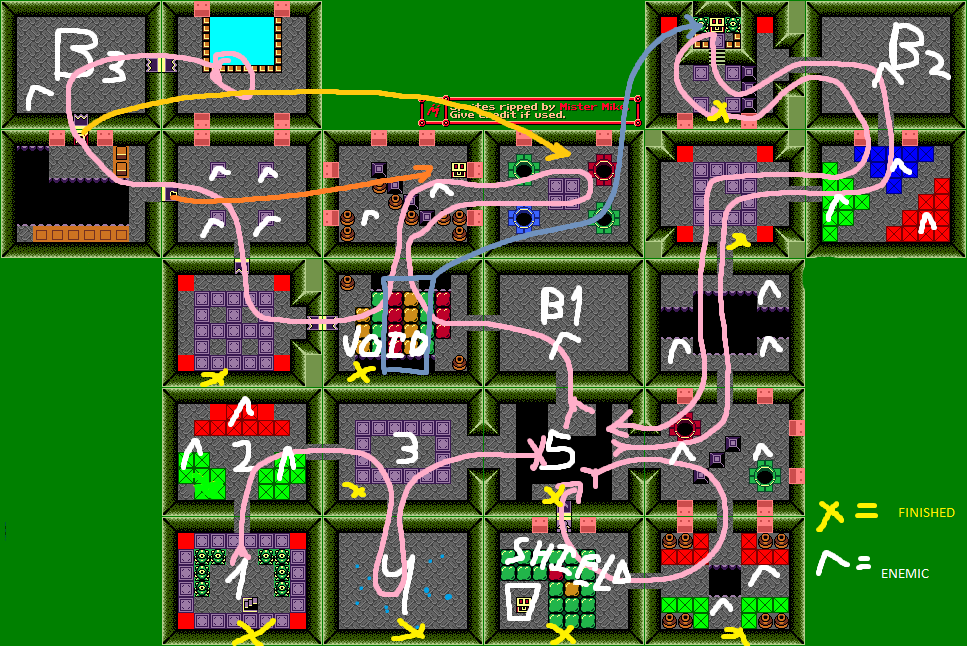
\includegraphics[width=0.8\textwidth]{../imgs/recorregut.png} % Example of adding a figure
    \caption{Mapa del joc amb el recorregut i els requerriments per a  cada nivell.}
    \label{fig:mapa}
\end{figure}

\section{Disseny}
Per al disseny del joc no hem seguit un patró de disseny concret. El ``loop'' del joc incorpora una clase auxiliar que anomenada \textbf{gamestatemanager}. Aquesta conté una llista amb els estats necessaris. L'objectiu de gastar aquesta classe és poder anyadir i eliminar estats dinamicament. Per exemple, quan el jugador apreta ``escape'' i s'obre el menú, el que realment s'està fent és concatenar dos estats i sols permitir que el més alt en la jerarquia puga llegir els inputs i actualitzar-se en funció del temps. 

Cada estat es responsable del seu propi update, draw i inputs. Estan dissenyats de manera que poden ser creats i destruits sense afetar als elements globals del joc com els nivells o el jugador. El jugador es persistent encara que es surti del nivell (escape -> Exit -> Start) per aquesta mateixa raó.

\subsection{Detecció de colisions}
Els elements poseeixen una ``bounding box''. L'escena itera sobre els objectes i comprova si hi ha solapament. En cas de solapament, el moviment es revertit. Quan hi ha colisió s'executa onCollide(item) amb una referencia del objecte colisionat. Aquest sistema afecta tant al Player com als enemics i els projectils. Adicionalment hem anyadit altres tipus de colisions com el ``SteptOn'' que permiteix saber sobre que element es troba el jugador. 

Els atacs del jugador generen una bounding box enfront d'ell i es comproba si colisiona amb algun enemic o element interactiu. Si es detecta una collisió, s'execute ``onCollided'' de cada objecte.


\subsection{Nivells, elements i entitats}
La classe \texttt{World} guarda un diccionari amb els mapes. La classe \texttt{Mapa} conté una llista amb els nivells. La classe \texttt{Level} contente una llista amb els elements i entitats que s'han de carregar. Per al projecte s'ha creat un World que conte dos mapes, ``dungeon1'' i ``overworld''. El mapa ``dungeon1'' conté 29 nivells. Cada nivell es responsable de contindre els estats per defecte de les entitats i també de customitzar events com "entrar" i "sortir" de les entitats. 

Scene es encarregada d'actualitzar els elements en cada fotograma. En primer lloc, Scene demana a World el contingut del nivell en el que es troba el jugador. A continuació, guarda una copia local d'aquests elements i permiteix al usuari interactuar amb ells. Tots els canvis que es realizen en els elements locals no es traslladen directament a la referencia global, sinó que s'actualitzen en funció de callbacks especials o per events externs. La naturaletza del joc requereix que els nivells tornen al seu estat original quan el jugador surt d'ells. Per això, implementar aquest comportament com el funcionament per defecte pareixia una idea acceptable. Aquesta estrategia comporta els seus inconvenients, com tindre que crear moltes funcions auxiliars per a comprtaments especifics o tindre que crear copies que influencien en la memoria del joc. 


\begin{figure}[ht!]
    \centering
    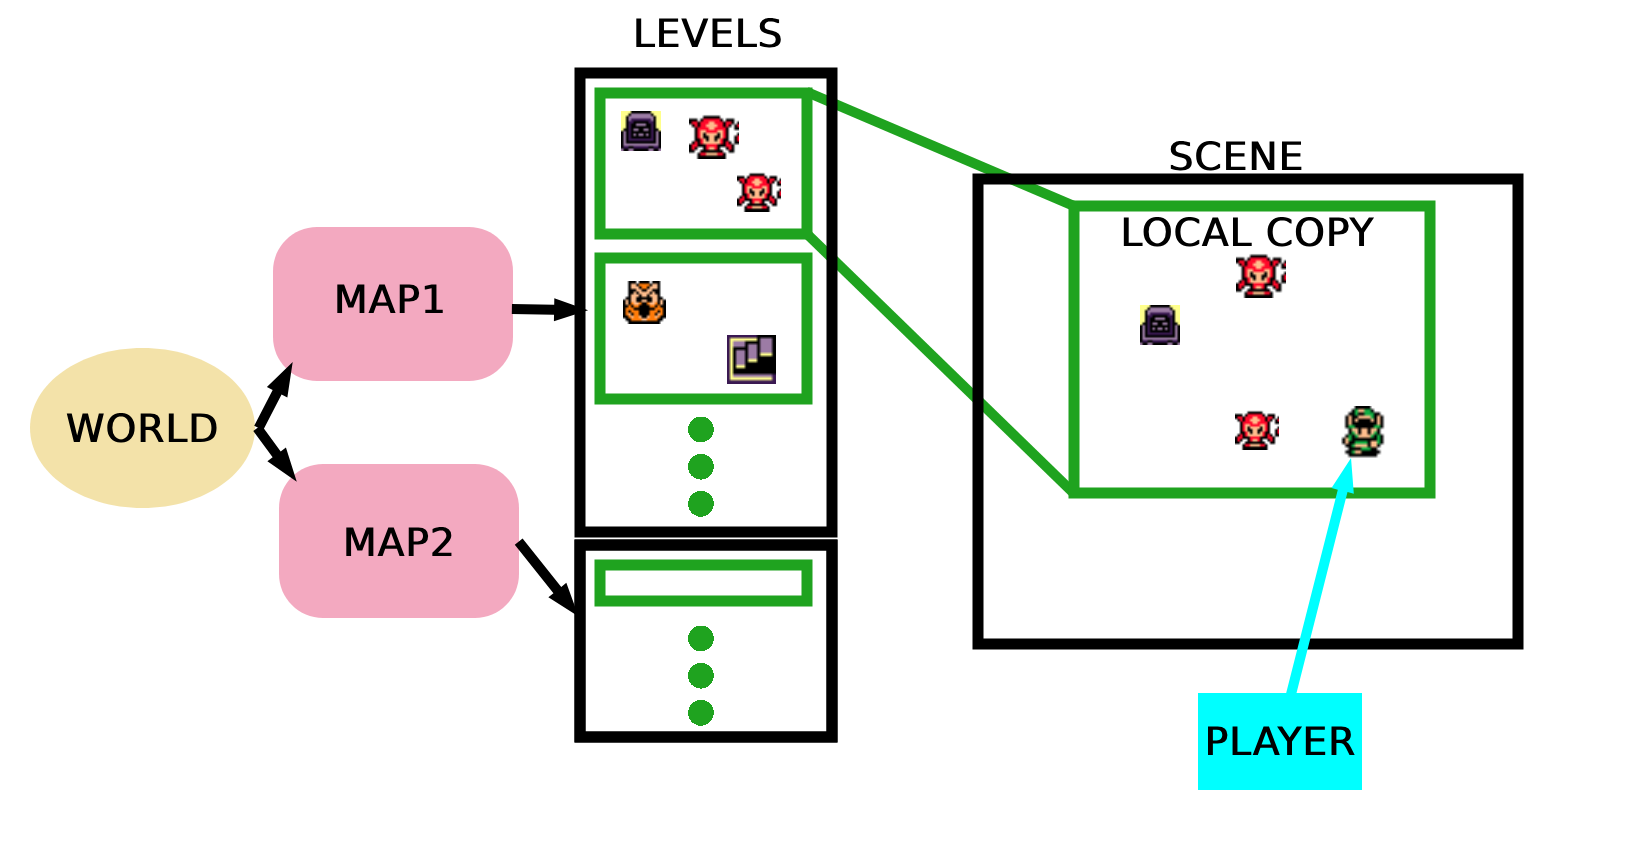
\includegraphics[width=0.8\textwidth]{../imgs/global_to_local.png} % Example of adding a figure
    \caption{Jerarquia dels elements durant l'execució del joc.}
    \label{fig:global_to_local}
\end{figure}

\subsubsection{Categories d'elements i entitats}

A continuació es mostren les diferents categories d'elements i entitats presents al joc, juntament amb exemples de cada tipus:

\begin{itemize}
    \item \textbf{Items equipables}
    \begin{itemize}
        \item Espasa
        \item Escut
        \item Ploma (Feather)
        \item Braçalet (Bracelet)
    \end{itemize}
    \item \textbf{Items}
    \begin{itemize}
        \item Claus
    \end{itemize}
    \item \textbf{Blocs}
    \begin{itemize}
        \item Blocks invisibles.
        \item Portcullis: portes que s'obrin i tanquen per scripts.
        \item Lights: block decoratiu animat.
        \item Vase: block decoratiu animat.
        \item Fire Place: block decoratiu animat.
        \item Animated Floor: block decoratiu animat.
    \end{itemize}
    \item \textbf{Blocs interactius}
    \begin{itemize}
        \item Sòls flotants (també representen el buit): es trenquen al passar per damunt.
        \item Làpides: es poden empentar.
        \item Cofres: es poden obrir i contenen objectes.
        \item Rotors: trenca closques que es poden resoldre al colpejar-los.
        \item Portes: es poden obrir amb claus.
        \item Portes en el pis: Teletransporten al jugador a un altre nivell.
        \item Estatua: Activa un dialeg.
        \item Floating Heart: Consumible que incrementa la vida del jugador.
        \item Floating Money: Consumible que incrementa la quantitat de diners del jugador.
    \end{itemize}
    \item \textbf{Entitats}
    \begin{itemize}
        \item Jugador
        \item Enemics comuns (slimes, ratpenats, etc.)
        \item Bosses
        \item NPCs
    \end{itemize}
\end{itemize}

\subsection{Mecàniques}
\subsubsection{Equipar Items}
Els items poseeixen atributs o effectes necessaris per a resoldre trenca closques o per a poder accedir a nivells. El objectes s'equipen mitjançant l'inventari.
\subsubsection{Atacar}
Atacar es un altra mecanica del joc. El jugador pot atacar als enemics i a alguns objectes.  
\subsubsection{Interactuar}
Alguns objectes com portes o estatues poden ser interactuats amb la tecla principal. Els objectes responen a l'interacció executant un callback. 
\subsubsection{Tocar}
Gracies a la detecció de colisions, podem ejecutar callbacks en funció de quin objecte esta colisionant amb el jugador. Per exemple, trencar el pis o empentar un objecte.

\subsection{Triggers}
Els levels poden contenir els següents triggers: 
\begin{itemize}
    \item \textbf{onEnter}: s'executa quan el jugador entra al nivell. Permiteix anyadir enemics a l'escena, moure al personatge amb un script, o qualsevol altre acció que es vulga realitzar quan el jugador entra al nivell. Adicionalment permet saber si es la primera vegada que el jugador entra al nivell. 
    \item \textbf{onExit}: s'executa quan el jugador surt del nivell. S'utilitza sobretot per a moure el personatge a una posició concreta.
    \item \textbf{onAllEnemiesDead}: s'executa quan tots els enemics del nivell estan morts. Per defecte, es desbloqueja la porta de sortida del nivell.
\end{itemize}

Amb aquests triggers podem fer apareixer un ``boss'' una unica vegada

Per a més control, també podem anyadir triggers personalitzats tant als objectes com als nivells. Normalment son utilitzats per a modificar l'estat d'un objecte permanentment.
\begin{itemize}
    \item \textbf{Tombstone}: La làpida de la cova de la mort té un trigger que es dispara quan el jugador la mou. Aquest trigger posiciona la làpida en una posició concreta de forma permanent.
\end{itemize} 

\section{Trenca closques}

\subsection{Lights Out}
Aquest trenca closques es basa en un joc de taula que consisteix a apagar totes les llums d'una graella. Cada vegada que es prem una llum, aquesta i les seves veïnes canvien d'estat (encenent-se si estaven apagades i apagant-se si estaven encenent-se). L'objectiu és trobar la combinació correcta de premudes per apagar totes les llums. 

Per a poder generar diferents trenca closques, s'ha creat una classe ``Rotor'' que contindrà: una id unica per nivell, una llista dels rotors als que afectarà (ids) i l'estat amb el que comença.

\begin{figure}[ht!]
    \centering
    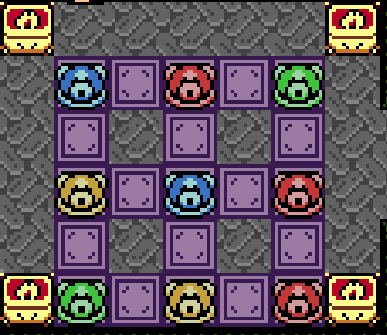
\includegraphics[width=0.6\textwidth]{../imgs/exemple-trencaclosques.png}
    \caption{Exemple visual d'un trenca-closques ``Lights Out'' implementat al joc.}
    \label{fig:exemple-trencaclosques}
\end{figure}

\subsection{Objectes Pesats}
Durant el joc, l'usuari es trobarà amb objectes que podrà empentar en algunes direccions. Aquest es el cas de les làpides i algunes pedres. Per a poder implementar aquest comportament, s'ha creat un item equipable (al igual que en el joc original) que incrementa les estadístiques de força del jugador. Si el jugador intenta desplaçar-se en una direcció constant i l'objecte obsstruint el pas es pot moure, aquest event es detectat per la classe \texttt{Player} i es realitza un moviment. 

Aques trenca closuqes bloqueja pantalles necessaries per a poder avançar en el joc:
\begin{itemize}
    \item Làpida de la cova de la mort: per a poder accedir a la cova de la mort, el jugador ha de moure una làpida que bloqueja l'entrada. Aquesta làpida es pot moure cap a dalt, baix i esquerra. En la mateixa cella on es trobava la làpida, hi ha una porta cap a la ``world.mapa['dungeon1']''
    \item Pedres pesades la vencer a ``B2'': hi ha que moureles per a poder accedir al cofre que conté la ``Feather'', objecte necessari per a volar.
\end{itemize}

\subsection{Preguntes i Respostes}
Algunes estatues poden requrir d'una resposta per part del jugador. La resposta activarà un trigger.


\section{Enemics}

\section{Menus}
Per a poder començar o eixir el joc, s'ha creat un conjunt de pantalles que permeten al jugador navegar per les opcions del joc. Aquestes pantalles es tracten com a estats del joc i es poden accedir mitjançant la tecla ``escape'' o alguns events.   
\begin{itemize}
    \item Start: Pantalla inicial del joc. Permet iniciar una partida o tancar el joc.
    \item Menu In Game: Pantalla que permet al jugador accedir als controls, reanudar o eixir del joc.
    \item Controls: Pantalla que mostra els controls del joc.
    \item Credits: Pantalla que mostra els crèdits del joc.
    \item Menu Final: Igual que el menú principal però amb una transició per a donar a entendre al jugador que ha guanyat.
    \item Dialegs: Encara que no són un ``menu'' en el sentit estricte, s'ha implementat un sistema de diàlegs que permet al jugador interactuar amb els NPCs i seleccionar diferent opcions.
\end{itemize}

\section{No Planejat}
La mort del jugador no esta implementada de forma que es considere part del loop jugable. Si la vida del personatge baixa al maxim, simplement apareix en alguna pantalla amb tot igual que abanç. Alguns triggers poden tenir problemes amb aquesta implementació. Si el jugador mor mentres lluita contra un ``boss'', la seguent vegada que entre pensarà que no es la primera vegada. La solució a aquest problema es poc elegant, però es soluciona fent varies comprobacions de si el boss ha sigut derrotat o no.






% \section{Examples}
% Code examples:
% \subsection{Text}
%  Lorem ipsum dolor sit amet, consectetur adipiscing elit. Donec sit amet arcu aliquam, mattis sapien quis, faucibus ligula. Praesent facilisis felis libero, nec scelerisque est vestibulum a. Proin gravida tempor neque eget maximus. Aliquam vel ex arcu. Maecenas porta blandit leo, eget dapibus libero faucibus quis. Curabitur vel sapien pharetra, ultricies nulla sed, ullamcorper metus. Sed mauris sapien, dapibus et elit in, bibendum pellentesque dui. Donec consequat quam ut pulvinar sodales. Duis commodo ex pharetra mauris dictum, in ultricies purus facilisis. Donec id ornare sem. Nam diam erat, imperdiet et orci id, lacinia condimentum justo. Integer laoreet pulvinar nibh. Vivamus vel tellus lacus.

% \begin{itemize}
%     \item one
%     \item one
%     \item one
%     \item one
%     \item one
    
% \end{itemize}

% Phasellus congue, massa in aliquet elementum, ipsum felis dictum enim, id maximus ante orci sit amet dui. Suspendisse blandit iaculis feugiat. Curabitur ante elit, tristique luctus hendrerit sed, posuere quis massa. Vivamus eu nunc vel neque egestas porttitor ac at nibh. Morbi odio justo, maximus sit amet elementum nec, finibus sed purus. Mauris eu posuere neque, at consequat elit. Praesent eu venenatis mauris, vel lobortis eros. Donec suscipit congue augue, ut aliquet metus volutpat ac. Vivamus mattis, nisl vel placerat euismod, tellus velit sollicitudin massa, nec sagittis nunc elit vel mauris. In id justo non nunc condimentum bibendum. Mauris scelerisque urna nisi, et lacinia justo posuere eget. 
% \begin{figure}[ht!]
%     \centering
%     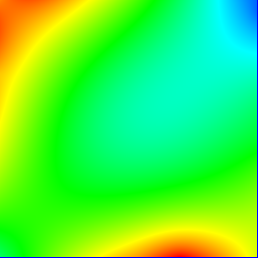
\includegraphics[width=0.8\textwidth]{img/eg.png} % Example of adding a figure
%     \caption{Test results for circuit 1}
%     \label{fig:circuit1}
% \end{figure}

% \begin{figure}[ht!]
%     \centering
%     \begin{minipage}{0.30\linewidth}
%         \centering
%         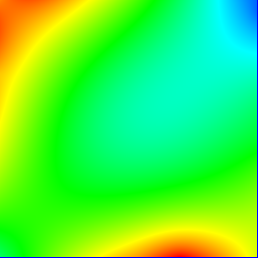
\includegraphics[width=\linewidth]{img/eg.png}
%         \caption{subimage1}
%         \label{fig:subimage1}
%     \end{minipage}
%     % \hfill
%     \begin{minipage}{0.30\linewidth}
%         \centering
%         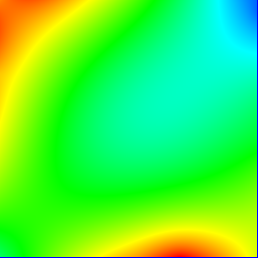
\includegraphics[width=\linewidth]{img/eg.png}
%         \caption{subimage2}
%         \label{fig:subimage2}
%     \end{minipage}
% \end{figure}


% \subsection{Code}
% \begin{minted}{c}
% #define NB 2 // selected based on the number of threads
% ...
% double relax_jacobi (double *u, double *utmp, unsigned sizex, unsigned sizey)
% {
% ...
%     #pragma omp parallel for reduction(+:sum) private(diff)
%     for (int ii=0; ii<nbx; ii++) {
%         ...
%     }
%     return sum;
% }
% \end{minted}

\newpage
% Bibliography (if required)
% Example citation to avoid warning
\nocite{*}
\bibliographystyle{plain}
\bibliography{references}  % Add a .bib file if you have references

\end{document}

\end{document}
